\chapter{Analiza wymagań}
Analiza wymagań to kluczowy etap procesu tworzenia oprogramowania. Ma on na celu zrozumienie potrzeb użytkowników oraz opracowanie poprawnej specyfikacji systemu. Oprócz wymagań funkcjonalnych, analiza powinna uwzględniać również aspekty związane ze skalowalnością, bezpieczeństwem i utrzymaniem systemu. W przypadku projektowania aplikacji istotne jest zidentyfikowanie wszystkich niezbędnych funkcji, które będą odpowiadały zarówno mieszkańcom, jak i administratorom. Ponadto, kluczowe będą: bezpieczeństwo, wydajność, intuicyjność interfejsu, architektura oraz integracja z innymi systemami.

\section{Architektura systemu} 
Zaprojektowanie architektury systemu przed jego implementacją umożliwia stworzenie efektywnego i funkcjonalnego rozwiązania. Proces projektowania architektury zazwyczaj rozpoczyna się od szkicowania jej zarysu, z wyszczególnieniem głównych komponentów systemu oraz ich wzajemnych interakcji. 

Na rysunku \ref{fig:zarys_architektury} przedstawiono zarys architektury projektowanego systemu. Uwzględniono w nim współpracujące ze sobą komponenty, wdrożone przy użyciu technologii konteneryzacji. Konteneryzacja umożliwia izolację poszczególnych modułów, co sprzyja ich łatwej skalowalności oraz zarządzaniu.
\begin{figure}[ht]
    \centering
    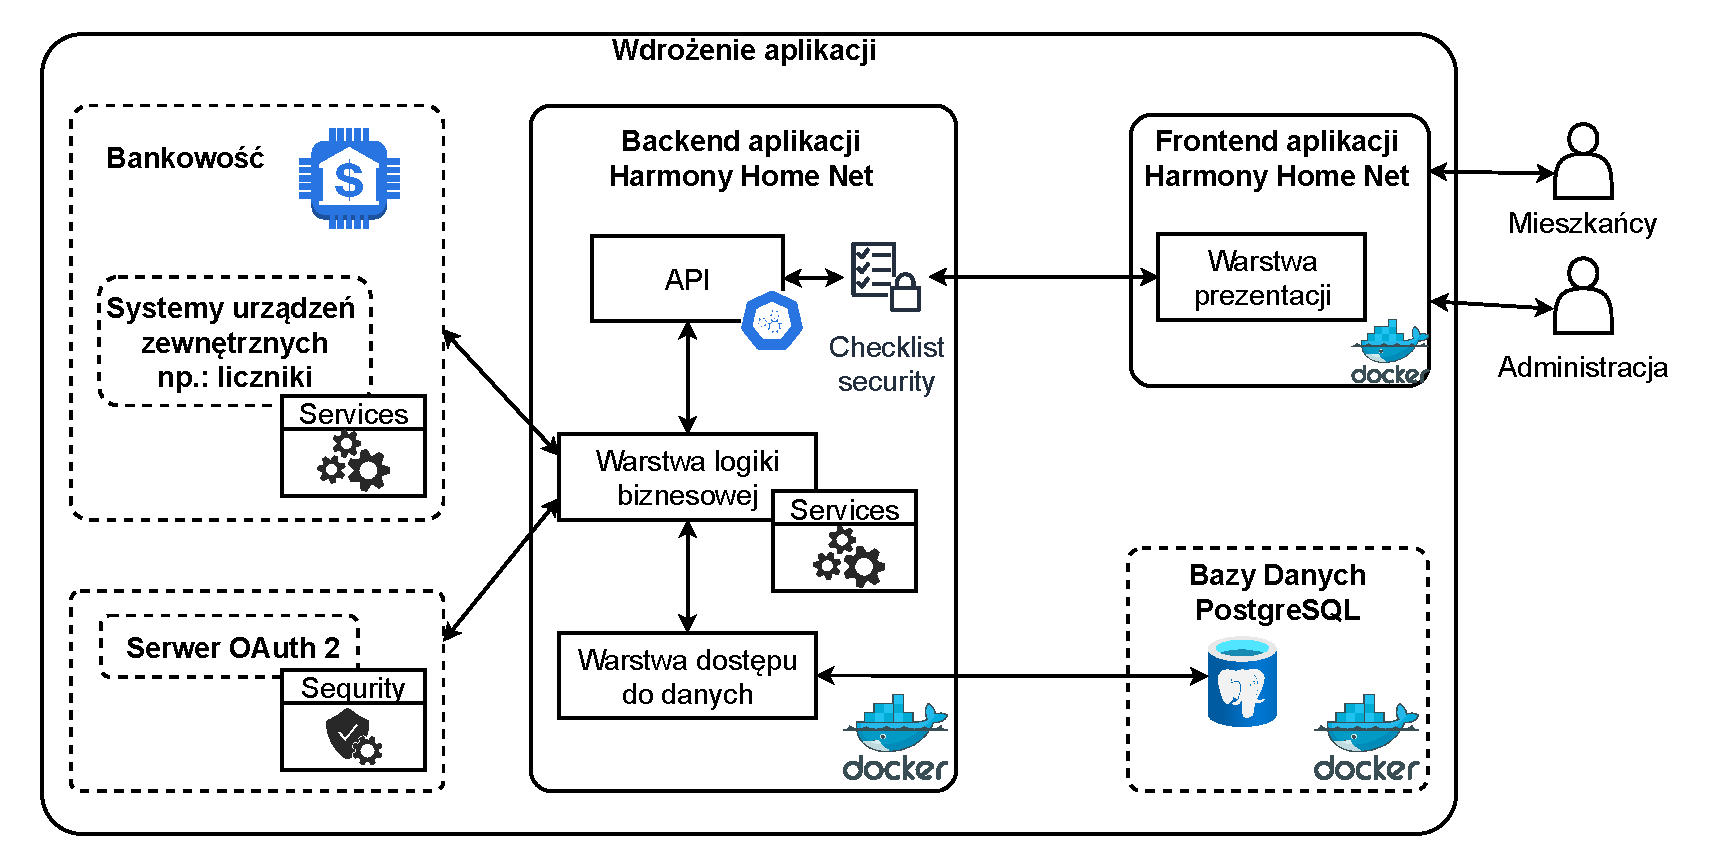
\includegraphics[width=.9\linewidth]{rys02/zarys_architektury}
    \caption{Zarys architektury systemu „Harmony Home Net”}
    \label{fig:zarys_architektury}
\end{figure}

\subsection{Komponenty systemu}
Zgodnie z tym, co przedstawiono na rysunku~\ref{fig:zarys_architektury}, system składa się z następujących elementów: 
% TO DO: przypominam o regułach związanych z kropkami na końcach zdań i przy skrótach - mówiłem o tym na spotkaniu on-line!!!
\begin{itemize}

    \item \textbf{Interfejs użytkownika (Frontend)} -- jest warstwą prezentacyjną aplikacji, zrealizowaną przy użyciu frameworka Next.js (TypeScript), odpowiedzialną za interakcje z użytkownikami oraz prezentację danych. Na rysunku~\ref{fig:zarys_architektury} frontend został umieszczony po prawej stronie, gdzie obsługuje mieszkańców oraz pracowników. Komunikacja z backendem odbywa się przy użyciu protokołu HTTP. Frontend jest również uruchamiany w kontenerze Dockerowym, co zapewnia jego izolację i ułatwia wdrożenie w środowiskach produkcyjnych.

    \item \textbf{Serwer (Backend)} -- to centralny moduł aplikacji, oparty na Spring Boot i~ uruchamiany w kontenerze Docker. Zarządza on logiką biznesową oraz przetwarzaniem danych. Na rysunku~\ref{fig:zarys_architektury}) backend znajduje się w centrum i pośredniczy między interfejsem użytkownika, bazą danych i zewnętrznymi systemami. Odpowiada za takie zadania, jak autoryzacja użytkowników (OAuth 2.0), zarządzanie zgłoszeniami technicznymi oraz obsługę transakcji finansowych. Konteneryzacja przy użyciu Dockera zapewnia elastyczność oraz ułatwia skalowanie.

    \item \textbf{Logika biznesowa} -- pełni funkcję koordynatora procesów biznesowych, odpowiedzialnego za przepływ danych pomiędzy warstwami systemu, takimi jak interfejs użytkownika, baza danych oraz systemy zewnętrzne. Na rysunku~\ref{fig:zarys_architektury} jest wyraźnie wyodrębniona jako kluczowy element przetwarzania zgłoszeń technicznych, zarządzania danymi użytkowników oraz integracji z systemami zewnętrznymi.

    \item \textbf{Warstwa dostępu do danych} -- odpowiada za operacje na bazie danych PostgreSQL, która przechowuje kluczowe informacje dotyczące użytkowników, zgłoszeń oraz transakcji. Na rysunku~\ref{fig:zarys_architektury} system bazodanowy został umieszczony po prawej stronie i bezpośrednio połączony z modułem serwerowym, co umożliwia efektywne zarządzanie danymi.

    \item \textbf{System bazodanowy} -- jest elementem odpowiadającym za przechowywanie wszystkich danych przetwarzanych w systemie. Aplikacja korzysta z obrazu PostgreSQL uruchamianego w~kontenerze Docker. Na rysunku~\ref{fig:zarys_architektury} baza danych PostgreSQL stanowi kluczowy element infrastruktury. Konteneryzacja bazy danych pozwala na łatwe zarządzanie środowiskiem oraz zwiększa bezpieczeństwo i skalowalność~\cite{Docker-docs,vsupalov}.

    \item \textbf{Moduł autoryzacji (OAuth 2.0)} -- zapewnia bezpieczny dostęp do zasobów systemu. Jak pokazano na rysunku~\ref{fig:zarys_architektury}, moduł ten pełni kluczową rolę w komunikacji pomiędzy warstwą serwerową a użytkownikami, kontrolując uprawnienia i dostęp do danych.

    \item \textbf{Systemy zewnętrzne} -- obejmują zewnętrzne systemy, takie jak systemy bankowe czy urządzenia pomiarowe (np.\ liczniki zużycia mediów), z którymi integruje się aplikacja. W lewej części rysunku~\ref{fig:zarys_architektury} widoczna jest współpraca systemów zewnętrznych z backendem, co umożliwia wymianę danych za pośrednictwem API.
		
\end{itemize}  


\subsection{Interakcje między komponentami}
Interakcje między komponentami są kluczowe do poprawnego funkcjonowania całej aplikacji. Szczegóły tych interakcji opisano poniżej. 

\begin{itemize}

	\item \textbf{Interfejs użytkownika i Serwer} -- moduł prezentacyjny (interfejs użytkownika) komunikuje się z warstwą serwerową poprzez żądania HTTP. Na rysunku~\ref{fig:zarys_architektury}połączenie pomiędzy tymi dwoma komponentami posiada ikonę \texttt{Checklist security}, symbolizującą kontrolę ról i~uprawnień użytkowników do konkretnych zasobów serwera. Warstwa serwerowa przetwarza zapytania i odsyła odpowiedzi w formacie JSON.

	\item \textbf{Moduł serwerowy i baza danych} -- warstwa serwerowa łączy się z bazą danych PostgreSQL uruchomioną w kontenerze Docker. Na rysunku~\ref{fig:zarys_architektury} przedstawiono to jako bezpośrednie połączenie między komponentami, co umożliwia efektywne wykonywanie operacji odczytu i zapisu danych.

	\item \textbf{Zarządzanie płatnościami} -- moduł serwerowy integruje się z systemami płatności, zapewniając obsługę transakcji finansowych. Widać to na rysunku~\ref{fig:zarys_architektury} po lewej stronie, gdzie systemy płatności wymieniają dane z warstwą serwerową, umożliwiając aktualizację statusu transakcji w bazie danych.

	\item \textbf{Powiadomienia dla użytkowników} -- powiadomienia są generowane bezpośrednio przez serwer i przesyłane do interfejsu użytkownika jako proste informacje, np. o zgłoszeniach, płatnościach lub głosowaniach. Na rysunku~\ref{fig:zarys_architektury} komunikację tę przedstawiono jako przepływ danych między serwerem, a interfejsem użytkownika, umożliwiając informowanie użytkowników o istotnych wydarzeniach w aplikacji.
	
\end{itemize}


\section{Wymagania aplikacji}

Aplikacja eBOK ma za zadanie wspierać zarządzanie wspólnotami mieszkaniowymi poprzez poprawę komunikacji między mieszkańcami a administracją oraz automatyzację procesów związanych z obsługą nieruchomości. Kluczowym elementem systemu jest zarządzanie lokalami, które odgrywają centralną rolę w wielu funkcjach aplikacji – od zgłaszania usterek, przez płatności, aż po organizację głosowań.

Lokale, definiowane jako nieruchomości (mieszkania, apartamenty, biura itp.), są głównym zasobem, który wymaga skutecznego zarządzania zarówno z perspektywy mieszkańca, jak i administracji spółdzielni oraz administratorów całego systemu. Mieszkaniec, będący właścicielem lokalu, przypisuje do swojego konta lokal, który jest podstawą do wszelkich interakcji z systemem, takich jak płatności, zgłoszenia techniczne czy udział w głosowaniach. Z kolei pracownicy administracji spółdzielni zarządzają bieżącymi operacjami dotyczącymi lokali, a administratorzy systemu mają pełen dostęp do wszystkich funkcji zarządzania aplikacją oraz integracji z~innymi systemami.

\subsection{Przykłady użycia aplikacji}

Aplikacja eBOK oferuje szeroki zakres funkcji, z których korzystają trzy główne grupy użytkowników. Wymieniono je poniżej. Każda z tych grup użytkowników korzysta z funkcji dostosowanych do ich potrzeb. Główne przypadki użycia obejmują zarządzanie relacjami pomiędzy mieszkańcami a administracją, w zakresie takich działań jak płatności, zgłoszenia usterek, dostęp do dokumentów oraz udział w głosowaniach. 
\begin{itemize} 

	\item \textbf{Mieszkańcy (właściciele)}: Po zalogowaniu do systemu, właściciele lokali mają możliwość przeglądania należności przypisanych do lokalu, regulowania opłat online oraz przeglądania historii rachunków. Mogą również zgłaszać usterki (np. awarie ogrzewania, przecieki) i monitorować status zgłoszeń. Mają pełen dostęp do dokumentów związanych z lokalem, takich jak umowy, regulaminy czy faktury. Oprócz tego mogą uczestniczyć w głosowaniach organizowanych przez administrację.
	
	\item \textbf{Pracownicy administracji spółdzielni}: Pracownicy administracji korzystają z panelu zarządzania spółdzielnią, który umożliwia im monitorowanie zgłoszeń technicznych, przypisywanie zadań wykonawcom oraz monitorowanie bieżących płatności dla lokali. Mają także możliwość organizowania i zarządzania głosowaniami mieszkańców oraz prowadzenia rejestru dokumentów związanych z lokalami.

	\item \textbf{Administratorzy systemu}: Administratorzy całego systemu mają dostęp do zaawansowanego panelu administracyjnego, który pozwala im na zarządzanie wszystkimi funkcjami aplikacji, w tym przypisywanie pracowników administracji do poszczególnych spółdzielni, monitorowanie działania systemu, konfigurowanie integracji z zewnętrznymi systemami oraz zarządzanie bazą danych lokali i użytkowników.

\end{itemize}



\subsection{Wymagania funkcjonalne}

Wymagania funkcjonalne aplikacji eBOK koncentrują się na kluczowych działaniach, które zapewniają sprawne funkcjonowanie wspólnot mieszkaniowych.

\begin{enumerate}[label=\arabic*.,labelwidth=\widthof{10}]

    \item \textbf{Zarządzanie kontem użytkownika i lokalami}: Każda grupa użytkowników posiada odrębne uprawnienia. Mieszkańcy mają możliwość zarządzania swoimi danymi oraz przypisywania lokali do konta. Pracownicy administracji mogą zarządzać kontami mieszkańców oraz przypisywać do nich lokale, a także zarządzać dokumentacją i zgłoszeniami dotyczącymi lokali. Administratorzy systemu zarządzają kontami wszystkich użytkowników, w tym pracowników administracji oraz mieszkańców.

	\item \textbf{Przegląd i płatność należności}: Właściciele lokali mogą przeglądać szczegóły dotyczące należności oraz historię płatności, a także realizować płatności online. System automatycznie wysyła powiadomienia o zaległościach, przypominając o konieczności uregulowania opłat. Pracownicy administracji mogą monitorować płatności wszystkich mieszkańców, przeglądać zaległości i zarządzać procesem windykacji. Administratorzy systemu mogą konfigurować integrację z systemami płatności oraz generować raporty dotyczące płatności.

	\item \textbf{Zarządzanie zgłoszeniami technicznymi dla lokali}:Mieszkańcy mogą zgłaszać usterki lub problemy techniczne związane ze swoimi lokalami oraz monitorować status tych zgłoszeń. Pracownicy administracji monitorują zgłoszenia, przypisują je odpowiednim wykonawcom i śledzą postęp napraw. Administratorzy systemu mogą zarządzać zgłoszeniami na poziomie globalnym, przeglądać ich historię i tworzyć raporty.

	\item \textbf{Zarządzanie dokumentami}: Właściciele mają pełen dostęp do dokumentów związanych z ich lokalami, takich jak umowy, regulaminy czy faktury. Pracownicy administracji zarządzają dokumentami powiązanymi z lokalami, przypisując je odpowiednim mieszkańcom oraz dbając o ich aktualność. Administratorzy systemu mogą tworzyć nowe kategorie dokumentów, zarządzać dostępami i monitorować całość systemu dokumentacji.

	\item \textbf{Głosowania mieszkańców}: Właściciele mogą brać udział w głosowaniach dotyczących spraw wspólnoty mieszkaniowej. Pracownicy administracji organizują głosowania, publikują wyniki i zarządzają całością procesu głosowania. Administratorzy systemu mają dostęp do statystyk i wyników głosowań oraz mogą nadzorować ich przebieg.
	
	\item \textbf{Powiadomienia i komunikacja}: System wysyła powiadomienia do mieszkańców o ważnych wydarzeniach, takich jak zaległe płatności, zgłoszenia serwisowe, planowane prace konserwacyjne czy nadchodzące głosowania. Pracownicy administracji mogą zarządzać powiadomieniami, konfigurować harmonogram wysyłki oraz komunikować się z mieszkańcami za pomocą różnych kanałów (e-mail, SMS). Administratorzy systemu mogą monitorować i konfigurować system powiadomień.
	
	\item \textbf{Panel administracyjny}: Pracownicy administracji korzystają z panelu, który umożliwia zarządzanie lokalami, przypisywanie mieszkańców, monitorowanie zgłoszeń technicznych i kontrolowanie płatności. Administratorzy systemu mają dostęp do zaawansowanych funkcji, takich jak zarządzanie całą bazą danych lokali, użytkowników, dokumentów oraz konfiguracja integracji z zewnętrznymi systemami.
	
	\item \textbf{Integracja z zewnętrznymi systemami}: Aplikacja eBOK integruje się z zewnętrznymi systemami, takimi jak systemy pomiarowe liczników mediów (np. wodomierze, liczniki energii) oraz platformy płatności. Integracja umożliwia automatyczne generowanie rachunków oraz synchronizację danych dotyczących zużycia mediów. Administratorzy systemu są odpowiedzialni za konfigurację i monitorowanie tych integracji.
	
	\item \textbf{Stany liczników}: Mieszkańcy mogą przeglądać stany liczników powiązanych z ich lokalami, takich jak wodomierze czy liczniki energii. Na podstawie wprowadzonych odczytów system automatycznie generuje rozliczenia. Pracownicy administracji mogą monitorować i weryfikować stany liczników oraz generować raporty rozliczeń dla całej wspólnoty. Administratorzy systemu zarządzają całą infrastrukturą liczników oraz integracją z systemami pomiarowymi.
	
	\item \textbf{Forum mieszkańców}: Mieszkańcy mogą korzystać z forum, aby dyskutować na tematy związane z zarządzaniem wspólnotą, zadawać pytania oraz dzielić się informacjami. Pracownicy administracji mogą moderować forum, odpowiadać na pytania mieszkańców oraz publikować ogłoszenia. Administratorzy systemu mają możliwość zarządzania strukturą forum, przypisywania moderatorów oraz nadzorowania aktywności na forum.
	
\end{enumerate}

\subsection{Wymagania niefunkcjonalne}

\begin{enumerate}[label=\arabic*.,labelwidth=\widthof{10}]

   \item \textbf{Skalowalność}: System musi być elastyczny, aby obsługiwać zarówno małe wspólnoty, jak i duże spółdzielnie, zarządzające setkami lub tysiącami lokali. Zastosowanie technologii Docker do konteneryzacji umożliwia skalowanie poziome (dodawanie instancji), co pozwala na efektywne rozdzielenie obciążenia.

	\item \textbf{Bezpieczeństwo}: Wszystkie dane muszą być przechowywane i przesyłane w sposób bezpieczny. Autoryzacja za pomocą OAuth 2.0. System musi także chronić dane przed nieautoryzowanym dostępem i atakami, np. SQL Injection czy XSS.

	\item \textbf{Wydajność}: System powinien zapewniać szybki czas odpowiedzi, szczególnie podczas przetwarzania dużych ilości danych, takich jak zgłoszenia techniczne czy płatności. Warstwa serwerowa oparta na Spring Boot oraz baza danych PostgreSQL muszą być odpowiednio zoptymalizowane.

	\item \textbf{Dostępność}: Aplikacja powinna być dostępna przez 99,9\% czasu, z minimalnymi przerwami na konserwację. Monitorowanie serwerów oraz wdrożenie technologii Docker umożliwia szybkie przywracanie usług w przypadku awarii.

	\item \textbf{Intuicyjność interfejsu}: Aplikacja musi być łatwa w obsłudze zarówno dla mieszkańców, jak i administratorów. Interfejs oparty na komponentach Shadcn UI, zgodny z WCAG 2.0, zapewnia dostępność i łatwość nawigacji.

	\item \textbf{Zgodność z przepisami RODO}: System musi spełniać wymagania RODO dotyczące ochrony danych osobowych. Użytkownicy muszą mieć możliwość wglądu w swoje dane, ich modyfikacji oraz usunięcia. Proces przetwarzania danych musi być udokumentowany, a dostęp do danych ograniczony.

	\item \textbf{Niezawodność}: System musi zapewniać ciągłość działania oraz regularne tworzenie kopii zapasowych bazy danych. Plan odzyskiwania po awarii musi umożliwiać szybkie przywrócenie funkcjonalności systemu.

	\item \textbf{Testowalność}: Wszystkie funkcje aplikacji powinny być testowane automatycznie, co pozwala na szybką identyfikację błędów. Testy jednostkowe, integracyjne i systemowe powinny obejmować zarówno warstwę serwerową, jak i interfejs użytkownika.

	\item \textbf{Elastyczność}: Architektura systemu musi umożliwiać łatwe wprowadzanie nowych funkcji oraz modyfikacje istniejących, bez konieczności szerokiej przebudowy kodu. Architektura warstwowa (N-tier) zapewnia rozdzielenie logiki biznesowej, danych oraz interfejsu użytkownika.

\end{enumerate}

\section{Podsumowanie}

Analiza wymagań dla systemu ,,Harmony Home Net’’ stanowi kluczowy krok w kierunku zaprojektowania i wdrożenia aplikacji, która sprosta potrzebom mieszkańców oraz administratorów wspólnot mieszkaniowych. Omówione w tym rozdziale wymagania funkcjonalne i niefunkcjonalne wyznaczają solidną podstawę do dalszego projektowania i planowania architektury systemu, gwarantując wysoką wydajność, bezpieczeństwo oraz skalowalność.
